\documentclass{article}
\usepackage{amsfonts}
\usepackage{graphicx}
\usepackage{mathtools}
\title{Assignment 4: Relations, Functions and Introducction to SML}
\author{Ernesto Rodriguez}
\begin{document}
\maketitle

\section{Problem 1}

\begin{enumerate}

\item{
  
  \[
  f:\mathbb{R} \rightarrow \mathbb{R}:f(x):= \left\{ 
  \begin{array}{l l}
    x^2 & \quad \text{if x $\geq$ 2}\\
    3x-2 & \quad \text{if x $<$ 2}\\
  \end{array} \right.
  \]

  {\bf Injective: }The function is injective since there exists no two x values that return the same value. This is due to the fact that the function is always growing and has no minimum. The picture shows it:

  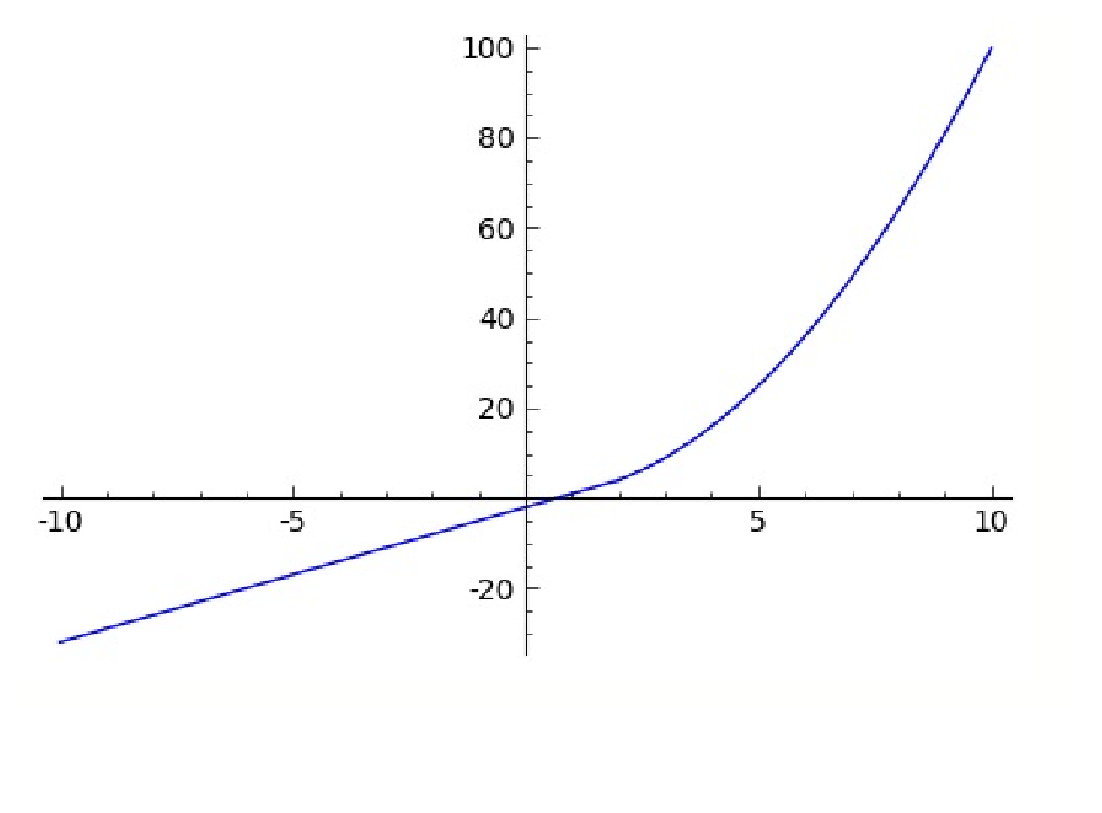
\includegraphics[width=100mm]{graph1.eps}

  {\bf Surjective: } The function is surjective because we can write the inverse function namely:

  \[
  f^{-1}:\mathbb{R} \rightarrow \mathbb{R}:f(x):= \left\{ 
  \begin{array}{l l}
    \sqrt{x} & \quad \text{if x $\geq$ 2}\\
    \frac{x+2}{3} & \quad \text{if x $<$ 2}\\
  \end{array} \right.
  \]

  This functions returns values that also belong to $\mathbb{R}$. Though $\sqrt{x}$ can be positive or negative, we are only using the positive part.

  {\bf Bijective: } This function is surjective and injective therefore is bijective.
  }

  \item{

    \[
    g: \mathbb{R} \rightarrow \mathbb{R},g(x):=2x^4 + 3x^3 + 4
    \]

    {\bf Injective: }This function isn't injective. As we can see on the graph, multiple values for x map the same y value.

    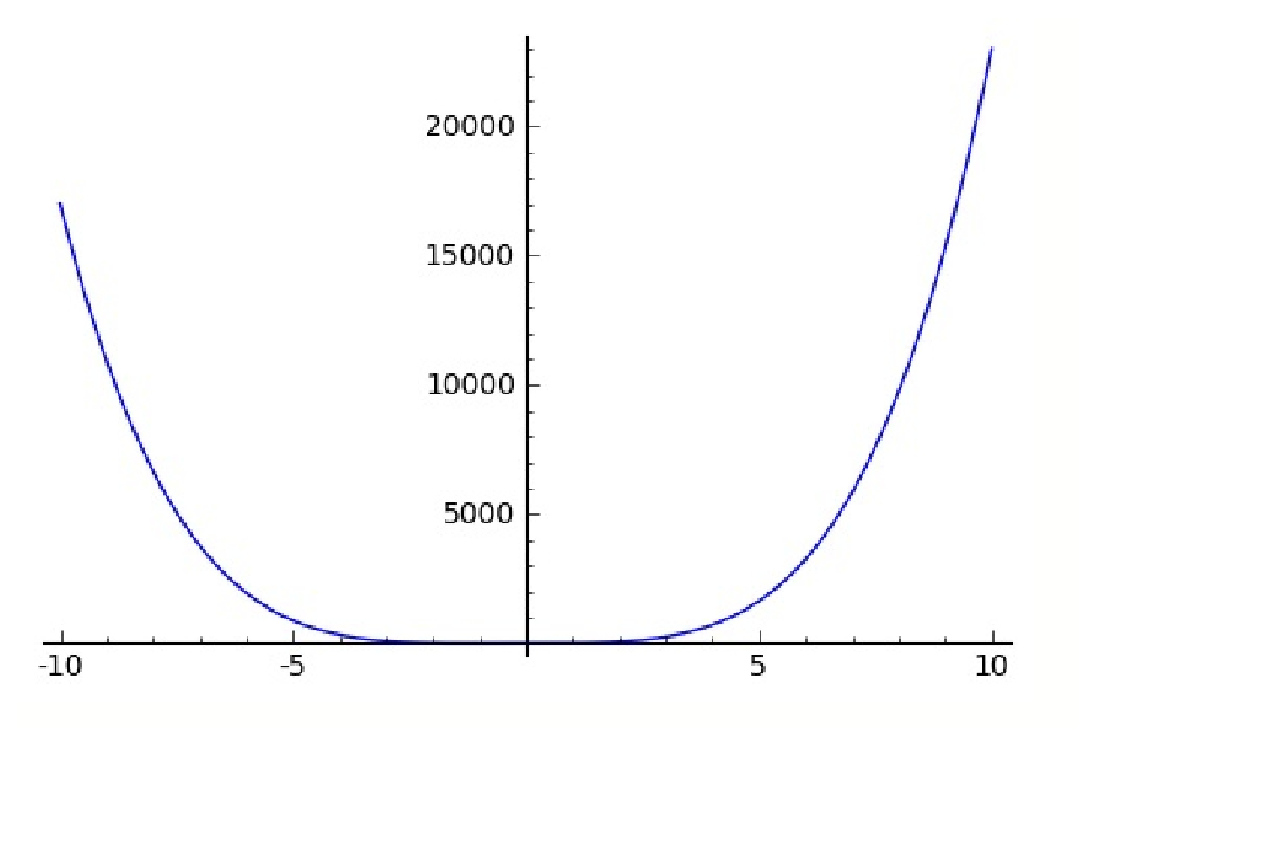
\includegraphics[width=100mm]{graph2.eps}

    {\bf Surjective: }This funciton isn't surjective since it dosen't have an image for all $\mathbb{R}$.

    {\bf Bijective: }This function isn't injective nor surjective so by definition it isn't bijective.

    }

\end{enumerate}
\end{document}
  
  
